\refstepcounter{chapter}
\addcontentsline{toc}{chapter}{Accessories}

\setsectiontitle{High-Speed Milling Spindle}
\setrevision{7631}

\setcounter{section}{2}

\subsection*{Application}
The high-speed milling spindle can be used in both the horizontal working spindle and the vertical working spindle of the machine.

\subsection*{Technical Data}
\begin{itemize}
    \item \textbf{Machine spindle taper} \dotfill ISO 40
    \item \textbf{Milling spindle internal taper} \dotfill ISO 30
    \item \textbf{Planetary gear ratio} \dotfill 1:4
    \item \textbf{Speed range} \dotfill 200-8000 RPM\footnotemark[1]
\end{itemize}

\subsection*{Anti-Rotation Protection}
\begin{itemize}
    \item The housing of the high-speed milling spindle is secured against rotation using a holding bracket (2) and a support rod (1).
    \item The support rod is fastened using a nut (3) at the required distance in the longitudinal slot of the holding bracket.
    \item The guide hole for mounting the support rod is located next to the machine spindle on the spindle head or on the vertical milling head.
\end{itemize}

\begin{figure}[h]
    \centering
    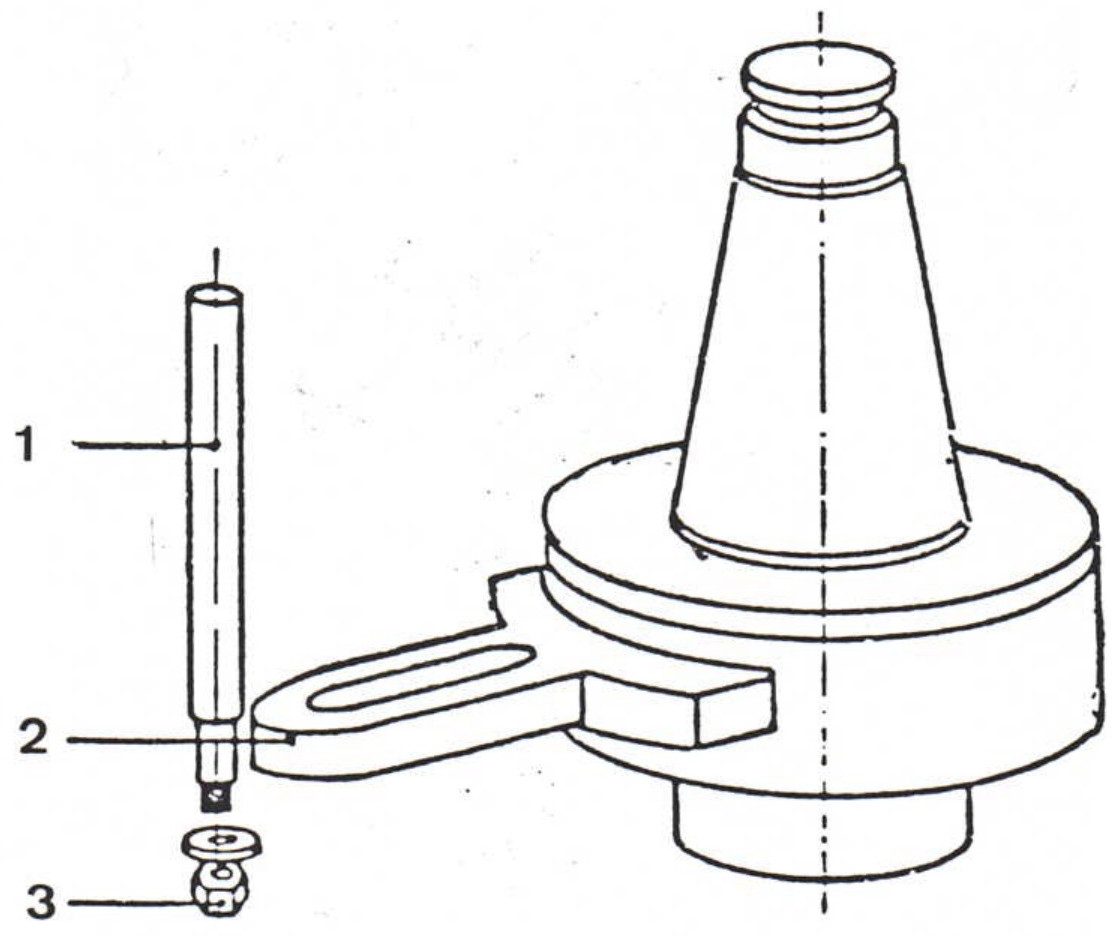
\includegraphics[width=0.7\textwidth]{chapter6/high_speed_milling_spindle.jpg}
\end{figure}

\footnotetext[1]{Maximum machine spindle speed: 2000 RPM.}
